\documentclass{article}\usepackage[]{graphicx}\usepackage[]{color}
%% maxwidth is the original width if it is less than linewidth
%% otherwise use linewidth (to make sure the graphics do not exceed the margin)
\makeatletter
\def\maxwidth{ %
  \ifdim\Gin@nat@width>\linewidth
    \linewidth
  \else
    \Gin@nat@width
  \fi
}
\makeatother

\definecolor{fgcolor}{rgb}{0.345, 0.345, 0.345}
\newcommand{\hlnum}[1]{\textcolor[rgb]{0.686,0.059,0.569}{#1}}%
\newcommand{\hlstr}[1]{\textcolor[rgb]{0.192,0.494,0.8}{#1}}%
\newcommand{\hlcom}[1]{\textcolor[rgb]{0.678,0.584,0.686}{\textit{#1}}}%
\newcommand{\hlopt}[1]{\textcolor[rgb]{0,0,0}{#1}}%
\newcommand{\hlstd}[1]{\textcolor[rgb]{0.345,0.345,0.345}{#1}}%
\newcommand{\hlkwa}[1]{\textcolor[rgb]{0.161,0.373,0.58}{\textbf{#1}}}%
\newcommand{\hlkwb}[1]{\textcolor[rgb]{0.69,0.353,0.396}{#1}}%
\newcommand{\hlkwc}[1]{\textcolor[rgb]{0.333,0.667,0.333}{#1}}%
\newcommand{\hlkwd}[1]{\textcolor[rgb]{0.737,0.353,0.396}{\textbf{#1}}}%

\usepackage{framed}
\makeatletter
\newenvironment{kframe}{%
 \def\at@end@of@kframe{}%
 \ifinner\ifhmode%
  \def\at@end@of@kframe{\end{minipage}}%
  \begin{minipage}{\columnwidth}%
 \fi\fi%
 \def\FrameCommand##1{\hskip\@totalleftmargin \hskip-\fboxsep
 \colorbox{shadecolor}{##1}\hskip-\fboxsep
     % There is no \\@totalrightmargin, so:
     \hskip-\linewidth \hskip-\@totalleftmargin \hskip\columnwidth}%
 \MakeFramed {\advance\hsize-\width
   \@totalleftmargin\z@ \linewidth\hsize
   \@setminipage}}%
 {\par\unskip\endMakeFramed%
 \at@end@of@kframe}
\makeatother

\definecolor{shadecolor}{rgb}{.97, .97, .97}
\definecolor{messagecolor}{rgb}{0, 0, 0}
\definecolor{warningcolor}{rgb}{1, 0, 1}
\definecolor{errorcolor}{rgb}{1, 0, 0}
\newenvironment{knitrout}{}{} % an empty environment to be redefined in TeX

\usepackage{alltt}

% Packages and Settings for LaTeX
\input{"C:/Users/Beniamino/Desktop/Mini_Project_1/Code/definitions"}

\title{\textbf{On Bootstrapping Spectral Estimates}}
\author{Beniamino Hadj-Amar}
\IfFileExists{upquote.sty}{\usepackage{upquote}}{}
\begin{document}

\maketitle

\renewenvironment{knitrout}{\vspace{1em}}{\vspace{1em}}



\section*{Setting the frequency}
Regardind setting the frequency, without messing up. This is true when $n$ is even.
\begin{knitrout}\footnotesize
\definecolor{shadecolor}{rgb}{0.969, 0.969, 0.969}\color{fgcolor}\begin{kframe}
\begin{alltt}
\hlcom{# Regarding the frequencies:}
\hlstd{n} \hlkwb{<-} \hlkwd{length}\hlstd{(data)}
\hlstd{n.tilda} \hlkwb{<-} \hlstd{n}\hlopt{/}\hlnum{2}
\hlstd{k} \hlkwb{<-} \hlnum{0}\hlopt{:}\hlstd{(n.tilda} \hlopt{-} \hlnum{1}\hlstd{)}
\hlstd{freq.rad} \hlkwb{<-} \hlnum{2}\hlopt{*}\hlstd{pi}\hlopt{*}\hlstd{k}\hlopt{/}\hlstd{n}
\hlstd{freq} \hlkwb{<-} \hlstd{k}\hlopt{/}\hlstd{n}

\hlcom{# Finding the period:}
\hlcom{# Let's say that I has a pick at position 13, the relative period is given by}
\hlnum{1}\hlopt{/}\hlstd{freq[}\hlnum{13}\hlstd{]}
\hlnum{2}\hlopt{*}\hlstd{pi}\hlopt{/}\hlstd{(freq.rad[}\hlnum{13}\hlstd{])}

\hlcom{# Also remember to set I(0) = 0}
\end{alltt}
\end{kframe}
\end{knitrout}


\section{Periodogram and Smoothed Periodogram}

Consider a discrete-time, real-valued stationary time series $\{X_t\}_{t \geq 1}$. Let's consider realisations $x_1, \dots, x_n$ of the process $\{X_t\}_{t \geq 1}$. For simplicity we assume that $n$ is even, and define $\widetilde{n}$ = $n/2$.
The periodogram is the Fourier transform of the empirical autocovariance function and can be written as:

\begin{equation*}
I(\omega_k) = \dfrac{1}{2\pi} | \sum_{t = 1}^{n} x_t \, \text{exp}(-i \omega_k t) |^2,
\end{equation*}
where $\omega_k$ = 2$\pi$k/$n$, k = 1, $\dots, \widetilde{n}$.

The code to compute the periodogram, given a time series is given below:

\begin{knitrout}\footnotesize
\definecolor{shadecolor}{rgb}{0.969, 0.969, 0.969}\color{fgcolor}\begin{kframe}
\begin{alltt}
\hlcom{# Function: Periodogram}
\hlstd{periodogram} \hlkwb{<-} \hlkwa{function}\hlstd{(}\hlkwc{data}\hlstd{) \{}
  \hlstd{n} \hlkwb{<-} \hlkwd{length}\hlstd{(data)}
  \hlstd{I} \hlkwb{<-} \hlstd{(}\hlkwd{abs}\hlstd{(}\hlkwd{fft}\hlstd{(data))}\hlopt{^}\hlnum{2}\hlstd{)}\hlopt{/}\hlstd{(n}\hlopt{*}\hlnum{2}\hlopt{*}\hlstd{pi)}
  \hlkwd{return}\hlstd{(I)}
\hlstd{\}}
\end{alltt}
\end{kframe}
\end{knitrout}

The periodogram is a unbiased but inconsistent estimator of the frequency spectrum.
A consistent estimator is obtained through smoothing techniques by a kernel spectral estimate of the form 

\begin{equation}
\label{eq:smoothed_periodogram}
\boxed{
\hat{f}_{b}(\omega_k) = \dfrac{\sum_{j = -\tilde{n}}^{n - 1} K_b(\omega_j - \omega_k) I(\omega_j)}{\sum_{l= -\tilde{n}}^{n - 1}K_b(\omega_l - \omega_k)}
}
\end{equation}

where $K_b(x)$ is a (scaled) Gaussian kernel:

\begin{equation}
\label{eq:gaussian_kernel}
K_b(x) = \frac{1}{b}\frac{1}{\sqrt{2\pi}}\text{exp}\Big\{ \dfrac{(x/b)^2}{2}\Big\}
\end{equation}

\begin{knitrout}\footnotesize
\definecolor{shadecolor}{rgb}{0.969, 0.969, 0.969}\color{fgcolor}\begin{kframe}
\begin{alltt}
\hlcom{# Function: Gaussian Kernel}
\hlstd{gaussian.kernel} \hlkwb{<-} \hlkwa{function}\hlstd{(}\hlkwc{x}\hlstd{,} \hlkwc{b} \hlstd{=} \hlnum{1}\hlstd{,} \hlkwc{scaled} \hlstd{=} \hlnum{FALSE}\hlstd{) \{}

  \hlkwa{if}\hlstd{(scaled} \hlopt{==} \hlnum{TRUE}\hlstd{) \{}
    \hlstd{out} \hlkwb{<-} \hlstd{(}\hlnum{1}\hlopt{/}\hlstd{b)} \hlopt{*} \hlstd{(}\hlnum{1}\hlopt{/}\hlkwd{sqrt}\hlstd{(}\hlnum{2}\hlopt{*}\hlstd{pi))} \hlopt{*} \hlkwd{exp}\hlstd{(}\hlopt{-}\hlstd{((x}\hlopt{/}\hlstd{b)}\hlopt{^}\hlnum{2}\hlstd{)}\hlopt{/}\hlnum{2}\hlstd{)}
    \hlkwd{return}\hlstd{(out)}
  \hlstd{\}}

  \hlstd{out} \hlkwb{<-} \hlstd{(}\hlnum{1}\hlopt{/}\hlkwd{sqrt}\hlstd{(}\hlnum{2}\hlopt{*}\hlstd{pi))} \hlopt{*} \hlkwd{exp}\hlstd{(}\hlopt{-}\hlstd{(x}\hlopt{^}\hlnum{2}\hlstd{)}\hlopt{/}\hlnum{2}\hlstd{)}
  \hlkwd{return}\hlstd{(out)}
\hlstd{\}}
\end{alltt}
\end{kframe}
\end{knitrout}



Furthermore, $I(0) = 0$, and $I(\omega_{-k}) = I(\omega_k)$. The bandwith $b$ is a positive paramater that controls the amount of smoothing imposed over $I(\omega)$.

The code to compute the smoothed periodogram in \ref{eq:smoothed_periodogram} is given below:

\begin{knitrout}\footnotesize
\definecolor{shadecolor}{rgb}{0.969, 0.969, 0.969}\color{fgcolor}\begin{kframe}
\begin{alltt}
\hlcom{# Function: Smoothed periodogram for single frequency}
\hlstd{single.smoothed.periodogram} \hlkwb{<-} \hlkwa{function}\hlstd{(}\hlkwc{x}\hlstd{,} \hlkwc{I}\hlstd{,} \hlkwc{b}\hlstd{) \{}

  \hlcom{# Auxiliary useful variables}
  \hlstd{n} \hlkwb{<-} \hlkwd{length}\hlstd{(I)}
  \hlstd{n.tilda} \hlkwb{<-} \hlstd{n}\hlopt{/}\hlnum{2}
  \hlstd{k} \hlkwb{<-} \hlkwd{seq}\hlstd{(}\hlkwc{from} \hlstd{=} \hlopt{-}\hlstd{n.tilda,} \hlkwc{to} \hlstd{= n} \hlopt{-} \hlnum{1}\hlstd{)}
  \hlstd{I.aux} \hlkwb{<-} \hlkwd{c}\hlstd{(I[n.tilda}\hlopt{:}\hlnum{1}\hlstd{],} \hlnum{0}\hlstd{,  I[}\hlnum{1}\hlopt{:}\hlstd{(n} \hlopt{-} \hlnum{1}\hlstd{)])}
  \hlstd{freq.aux} \hlkwb{<-} \hlnum{2}\hlopt{*}\hlstd{pi}\hlopt{*}\hlstd{k}\hlopt{/}\hlstd{n}

  \hlcom{# Kernel coefficients}
  \hlstd{temp} \hlkwb{<-} \hlkwd{gaussian.kernel}\hlstd{(freq.aux} \hlopt{-} \hlstd{x, b,} \hlkwc{scaled} \hlstd{=} \hlnum{TRUE}\hlstd{)}

  \hlcom{# Evaluating smoothed periodogram}
  \hlstd{numerator} \hlkwb{<-} \hlstd{temp} \hlopt \hlstd{I.aux}
  \hlstd{denominator} \hlkwb{<-} \hlkwd{sum}\hlstd{(temp)}
  \hlstd{I.smoothed} \hlkwb{<-} \hlstd{numerator}\hlopt{/}\hlstd{denominator}

  \hlkwd{return}\hlstd{(I.smoothed)}
\hlstd{\}}

\hlcom{# Function: Smoothed periodogram}
\hlstd{smoothed.periodogram} \hlkwb{<-} \hlkwa{function}\hlstd{(}\hlkwc{freq}\hlstd{,} \hlkwc{I}\hlstd{,} \hlkwc{b}\hlstd{) \{}
  \hlstd{out} \hlkwb{<-} \hlkwd{c}\hlstd{()}
  \hlkwa{for}\hlstd{(i} \hlkwa{in} \hlnum{1}\hlopt{:}\hlkwd{length}\hlstd{(freq)) \{}
    \hlstd{out[i]} \hlkwb{<-} \hlkwd{single.smoothed.periodogram}\hlstd{(freq[i], I, b)}
  \hlstd{\}}
  \hlkwd{return}\hlstd{(out)}
\hlstd{\}}
\end{alltt}
\end{kframe}
\end{knitrout}

\subsection{Selecting the bandwith $b$}
The optimal value of the bandwith $b$ is $c \times n^{-1/5}$, for some positive constant $c$. It has been proposed to choose $b$ to minimise a risk function, which is an unbiased estimator of the residual sum of square.

\begin{equation}
\label{eq:RSS}
\hat{R}(b) = \sum_{k = 0}^{\tilde{n} - 1} \Big\{  I(\omega_k)  - \hat{f}_b(\omega_k)\Big\}^2 - \dfrac{1 - 2W_b}{2} \sum_{k = 0}^{\tilde{n} - 1} I(\omega_k)^2,
\end{equation}

where $W_b = K_b(0)/\sum_{j = -\tilde{n}}^{n - 1} K_b(\omega_j)$.

The code to compute \ref{eq:RSS} is given by

\begin{knitrout}\footnotesize
\definecolor{shadecolor}{rgb}{0.969, 0.969, 0.969}\color{fgcolor}\begin{kframe}
\begin{alltt}
\hlcom{### Function: unbiased estimate for Residual Sum of Squares (RSS)}
\hlstd{unbiased.RSS} \hlkwb{<-} \hlkwa{function}\hlstd{(}\hlkwc{b}\hlstd{,} \hlkwc{I}\hlstd{) \{}

  \hlcom{# n, \textbackslash{}tilde\{n\}}
  \hlstd{n} \hlkwb{<-} \hlkwd{length}\hlstd{(I)}
  \hlstd{n.tilda} \hlkwb{<-} \hlstd{n}\hlopt{/}\hlnum{2}
  \hlcom{# Frequencies}
  \hlstd{k} \hlkwb{<-} \hlnum{1}\hlopt{:}\hlstd{n.tilda}
  \hlstd{freq.rad} \hlkwb{<-} \hlnum{2}\hlopt{*}\hlstd{pi}\hlopt{*}\hlstd{k}\hlopt{/}\hlstd{n}

  \hlcom{# Smoothed.periodogram}
  \hlstd{I.smooth} \hlkwb{<-} \hlkwd{smoothed.periodogram}\hlstd{(freq.rad, I,} \hlkwc{b} \hlstd{= b)}

  \hlcom{# Auxiliary variables}
  \hlstd{k.aux} \hlkwb{<-} \hlkwd{seq}\hlstd{(}\hlkwc{from} \hlstd{=} \hlopt{-}\hlstd{n.tilda,} \hlkwc{to} \hlstd{= n} \hlopt{-} \hlnum{1}\hlstd{)}
  \hlstd{freq.aux} \hlkwb{<-} \hlnum{2}\hlopt{*}\hlstd{pi}\hlopt{*}\hlstd{k.aux}\hlopt{/}\hlstd{n}

  \hlcom{# Constant for bias}
  \hlstd{K.0} \hlkwb{<-} \hlkwd{gaussian.kernel}\hlstd{(}\hlnum{0}\hlstd{,} \hlkwc{b} \hlstd{= b,} \hlkwc{scaled} \hlstd{= T)}
  \hlstd{norm.const} \hlkwb{<-} \hlkwd{sum}\hlstd{(}\hlkwd{gaussian.kernel}\hlstd{(freq.aux,} \hlkwc{b} \hlstd{= b,} \hlkwc{scaled} \hlstd{= T))}
  \hlstd{W.b} \hlkwb{<-} \hlstd{K.0}\hlopt{/}\hlstd{norm.const}

  \hlcom{# RSS}
  \hlstd{RSS} \hlkwb{<-} \hlkwd{sum}\hlstd{((I[}\hlnum{1}\hlopt{:}\hlstd{n.tilda]} \hlopt{-} \hlstd{I.smooth)}\hlopt{^}\hlnum{2}\hlstd{)}
  \hlcom{# Bias}
  \hlstd{bias} \hlkwb{<-} \hlstd{((}\hlnum{1} \hlopt{-} \hlnum{2}\hlopt{*}\hlstd{W.b)}\hlopt{/}\hlnum{2}\hlstd{)} \hlopt{*} \hlkwd{sum}\hlstd{(I[}\hlnum{1}\hlopt{:}\hlstd{n.tilda]}\hlopt{^}\hlnum{2}\hlstd{)}
  \hlcom{# Unbiased estimate}
  \hlstd{out} \hlkwb{<-} \hlstd{RSS} \hlopt{-} \hlstd{bias}

  \hlkwd{return}\hlstd{(out)}
\hlstd{\}}
\end{alltt}
\end{kframe}
\end{knitrout}

In pratice to find $b$, we compute $\hat{R}(b)$ for a grid of value of $c$ (let's say between 0 and 1), and we select the value of $c$ which minimises this risk function. An example of this is given in the figure below, by using the dataset \texttt{sunspotz}.

\begin{figure}[htbp]
\centering
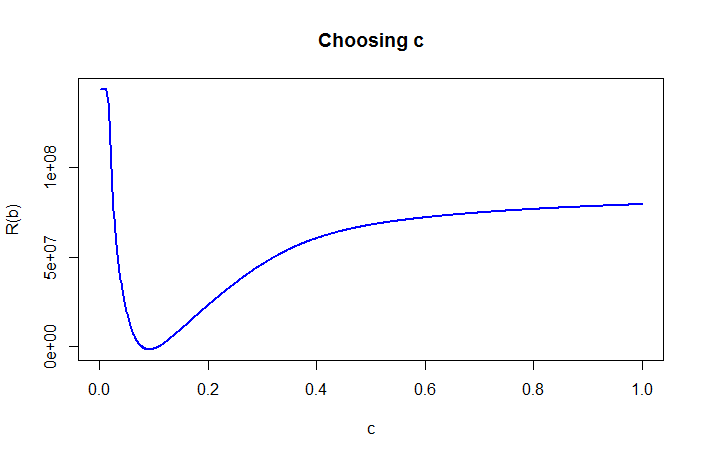
\includegraphics[scale = 0.2]{Plots/Choosing_c.png}
\end{figure}

To make the life easier we make a function to find the value of $c$, and we test the performance of the spectral smoothing, and the elictation of the bandwith. The code and the plots are given below:


\begin{knitrout}\footnotesize
\definecolor{shadecolor}{rgb}{0.969, 0.969, 0.969}\color{fgcolor}\begin{kframe}
\begin{alltt}
\hlkwd{source}\hlstd{(}\hlstr{"Kernel_Smoothing_Spectrum.R"}\hlstd{)}

\hlkwd{library}\hlstd{(astsa)}
\hlkwd{data}\hlstd{(}\hlstr{"sunspotz"}\hlstd{)}

\hlcom{# Testing on Sunspotz Data (considering n even)}
\hlstd{x} \hlkwb{<-} \hlkwd{as.vector}\hlstd{(sunspotz);}
\hlstd{x} \hlkwb{<-} \hlstd{x[}\hlopt{-}\hlnum{1}\hlstd{]}
\hlstd{n} \hlkwb{<-} \hlkwd{length}\hlstd{(sunspotz)}

\hlcom{# Frequency (radiant)}
\hlstd{n.tilda} \hlkwb{<-} \hlstd{n}\hlopt{/}\hlnum{2}
\hlstd{k} \hlkwb{<-} \hlnum{0}\hlopt{:}\hlstd{(n.tilda} \hlopt{-} \hlnum{1}\hlstd{)}
\hlstd{freq.rad} \hlkwb{<-} \hlnum{2}\hlopt{*}\hlstd{pi}\hlopt{*}\hlstd{k}\hlopt{/}\hlstd{n}

\hlcom{# Periodogram, and setting I(0) = 0}
\hlstd{I} \hlkwb{<-} \hlkwd{periodogram}\hlstd{(x)}
\hlstd{I[}\hlnum{1}\hlstd{]} \hlkwb{<-} \hlnum{0}

\hlcom{# Smoothed periodogram }
\hlcom{# Notice: to evaluate smoothed.periodogram we need to use freq.rad}
\hlstd{I.smooth} \hlkwb{<-} \hlkwd{smoothed.periodogram}\hlstd{(freq.rad, I,} \hlkwc{b} \hlstd{=} \hlnum{0.14}\hlstd{)}

\hlcom{# Plotting periodgram and smoothed periodogram}
\hlkwd{plot}\hlstd{(freq.rad, I[}\hlnum{1}\hlopt{:}\hlstd{(n.tilda)],} \hlkwc{type} \hlstd{=} \hlstr{"l"}\hlstd{)}
\hlkwd{lines}\hlstd{(freq.rad, I.smooth[}\hlnum{1}\hlopt{:}\hlstd{(n.tilda)],} \hlkwc{type} \hlstd{=} \hlstr{"l"}\hlstd{,}
      \hlkwc{col} \hlstd{=} \hlstr{"red"}\hlstd{,} \hlkwc{lwd} \hlstd{=} \hlnum{2}\hlstd{)}

\hlcom{# We want to find the c, for which the unbised RSS(b) is minimised.}
\hlstd{c} \hlkwb{<-} \hlkwd{find.c}\hlstd{(I)}
\hlstd{c;}

\hlcom{# Therefore the optimal b is given by:}
\hlstd{b} \hlkwb{<-} \hlstd{c} \hlopt{*} \hlstd{(n} \hlopt{^} \hlstd{(}\hlopt{-}\hlnum{1}\hlopt{/}\hlnum{5}\hlstd{)); b}
\hlstd{I.smooth} \hlkwb{<-} \hlkwd{smoothed.periodogram}\hlstd{(freq.rad, I,} \hlkwc{b} \hlstd{= b)}

\hlcom{# The plotted results:}
\hlkwd{plot}\hlstd{(freq.rad, I[}\hlnum{1}\hlopt{:}\hlstd{(n.tilda)],} \hlkwc{type} \hlstd{=} \hlstr{"l"}\hlstd{,} \hlkwc{ylab} \hlstd{=} \hlstr{"Power spectrum"}\hlstd{)}
\hlkwd{lines}\hlstd{(freq.rad, I.smooth[}\hlnum{1}\hlopt{:}\hlstd{(n.tilda)],} \hlkwc{type} \hlstd{=} \hlstr{"l"}\hlstd{,}
      \hlkwc{col} \hlstd{=} \hlstr{"red"}\hlstd{,} \hlkwc{lwd} \hlstd{=} \hlnum{2}\hlstd{)}
\end{alltt}
\end{kframe}
\end{knitrout}

where

\begin{knitrout}\footnotesize
\definecolor{shadecolor}{rgb}{0.969, 0.969, 0.969}\color{fgcolor}\begin{kframe}
\begin{alltt}
\hlcom{# Function: find c that minimise the unbised RSS}
\hlstd{find.c} \hlkwb{<-} \hlkwa{function}\hlstd{(}\hlkwc{I}\hlstd{) \{}

  \hlcom{# Length time series}
  \hlstd{n} \hlkwb{<-} \hlkwd{length}\hlstd{(I)}
  \hlcom{# Grid}
  \hlstd{c} \hlkwb{<-} \hlstd{(}\hlnum{1}\hlopt{:}\hlnum{1e3}\hlstd{)}\hlopt{/}\hlnum{1e3}
  \hlstd{b} \hlkwb{<-} \hlstd{c} \hlopt{*} \hlstd{(n}\hlopt{^}\hlstd{(}\hlopt{-}\hlnum{1}\hlopt{/}\hlnum{5}\hlstd{))}

  \hlcom{# Risk values}
  \hlstd{risk.values} \hlkwb{<-} \hlkwd{c}\hlstd{()}
  \hlkwa{for}\hlstd{(i} \hlkwa{in} \hlnum{1}\hlopt{:}\hlkwd{length}\hlstd{(c)) \{}
    \hlstd{risk.values[i]} \hlkwb{<-} \hlkwd{unbiased.RSS}\hlstd{(}\hlkwc{b} \hlstd{= b[i], I)}
  \hlstd{\}}

  \hlcom{# Values of C that minimises the risk value}
  \hlstd{out} \hlkwb{<-} \hlstd{c[}\hlkwd{which}\hlstd{(risk.values} \hlopt{==} \hlkwd{min}\hlstd{(risk.values))]}

  \hlkwd{return}\hlstd{(out)}
\hlstd{\}}
\end{alltt}
\end{kframe}
\end{knitrout}

The spectrum and the smoothed spectrum are given in Figure \ref{fig:spectrum_vs_smoothing}

\begin{figure}[htbp]
\centering
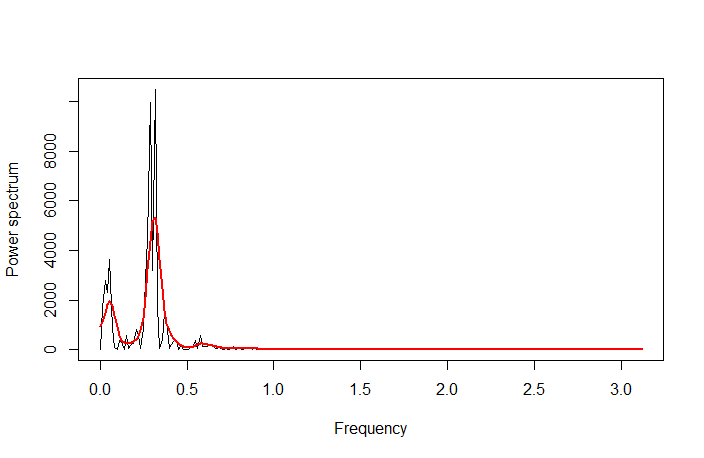
\includegraphics[scale = 0.4]{Plots/period_vs_smoothing.png}
\caption{Black line: periodogram; Red Line: smoothed spectrum, with $c$ = 0.091, and therefore $b$ = 0.0267}
\label{fig:spectrum_vs_smoothing}
\end{figure}


\section{Bootstrap Spectral Estimates}

Recall the important result $\dfrac{2 I(\omega_k)}{f(\omega_k)} \sim \chi^2(2) $. It follows immediately that

\begin{equation}
\label{eq:mult_reg}
I(\omega_k) = f(\omega_k) \epsilon_k, \quad \text{where } \epsilon_k \sim \text{Expo}(1).
\end{equation}

We use this relationship to interprete the spectral estimation problem as an approximate multiplicative regression problem.

We consider the following procedure for getting a bootstrap approximation of $\hat{f}_b(\omega_k)$. We define this method as \textit{Spectral Resampling} (SR).

\begin{itemize}

\item \textbf{Step 1}

We choose an initial bandiwth $b_{\dagger} = c \cdot n^{-1/4}$. We estimate the residuals $\hat{\epsilon}_k$, $k = 1,\dots, \tilde{n}$ of \ref{eq:mult_reg} as $$ \hat{\epsilon}_k = \dfrac{I(\omega_k)}{\hat{f}_{b_{\dagger}}(\omega_k)}, \quad k = 1, \dots, \tilde{n}$$


We rescale the empirical residuals by considering

$$ \tilde{\epsilon}_k =  \dfrac{\hat{\epsilon}_k}{\hat{\epsilon}}, \quad k = 1, \dots, \tilde{n}, \quad \text{where  } \hat{\epsilon} = \frac{1}{\tilde{n}} \sum_{j = 1}^{\tilde{n}} \tilde{\epsilon}_j$$

\item \textbf{Step 2}

We draw independent bootstrap residuals $\epsilon_1^{*}, \dots, \epsilon_{\tilde{n}}^{*}$ from the empirical distribution of $\tilde{\epsilon}_1, \dots, \tilde{\epsilon}_{\tilde{n}}$

Following \ref{eq:mult_reg} we define bootstrap periodogram values as

$$I^{*}(\omega_k) = I^{*}(\omega_{-k}) = \hat{f}_{b_{\ddagger}}(\omega_k) \epsilon^{*}_k, \quad k = 1, \dots, \tilde{n}$$,

where $b_{\ddagger} = c \cdot n^{-1/6}$. 

Finally we obtain a bootstrap spectral estimate as 
$$ \hat{f}^{*}_{b} (\omega) = \dfrac{\sum_{k = -\tilde{n}}^{n - 1} \Big\{ K_b(\omega_k - \omega) I^{*}(\omega_k) \Big\}}{\sum_{l = -\tilde{n}}^{n - 1} \Big\{ K_b(\omega_l - \omega) \Big\}} $$

where $b = c \cdot n^{-1/5}$. Notice that in order to evaluate $\hat{f}_{b_{\ddagger}}(\omega_k)$ for $k > \tilde{n}$, we use the fact that $$\hat{f}_{b_{\ddagger}}(\omega_{[\tilde{n} + k]}) = \hat{f}_{b_{\ddagger}}(\omega_{[\tilde{n} - k]}), \quad |k| > \tilde{n}.$$
\end{itemize}

We now give the code to implement the SR method.
We need a couple of functions to evaluate the final bootstrap spectral estimate:

\begin{knitrout}\footnotesize
\definecolor{shadecolor}{rgb}{0.969, 0.969, 0.969}\color{fgcolor}\begin{kframe}
\begin{alltt}
\hlcom{### Function: single estimate for bootstrap spectrum}
\hlstd{single.f.star} \hlkwb{<-} \hlkwa{function}\hlstd{(}\hlkwc{x}\hlstd{,} \hlkwc{I.smooth}\hlstd{,} \hlkwc{residuals}\hlstd{,} \hlkwc{b}\hlstd{) \{}

  \hlcom{# Setting length parameters}
  \hlstd{n} \hlkwb{<-} \hlkwd{length}\hlstd{(I.smooth)} \hlopt{*} \hlnum{2}
  \hlstd{n.tilda} \hlkwb{<-} \hlkwd{length}\hlstd{(I.smooth)}

  \hlcom{# Parameters}
  \hlstd{k} \hlkwb{<-} \hlkwd{seq}\hlstd{(}\hlkwc{from} \hlstd{=} \hlopt{-}\hlstd{n.tilda,} \hlkwc{to} \hlstd{= n} \hlopt{-} \hlnum{1}\hlstd{)}
  \hlstd{freq.aux} \hlkwb{<-} \hlnum{2}\hlopt{*}\hlstd{pi}\hlopt{*}\hlstd{k}\hlopt{/}\hlstd{n}

  \hlcom{# Auxiliary objects}
  \hlstd{residuals.aux} \hlkwb{<-} \hlkwd{c}\hlstd{(residuals[n.tilda}\hlopt{:}\hlnum{1}\hlstd{],} \hlnum{0}\hlstd{, residuals[}\hlnum{1}\hlopt{:}\hlstd{n.tilda],}
                     \hlstd{residuals[(n.tilda} \hlopt{-} \hlnum{1}\hlstd{)} \hlopt{:} \hlnum{1}\hlstd{])}
  \hlstd{I.smooth.aux} \hlkwb{<-} \hlkwd{c}\hlstd{(I.smooth[n.tilda}\hlopt{:}\hlnum{1}\hlstd{],} \hlnum{0}\hlstd{, I.smooth[}\hlnum{1}\hlopt{:}\hlstd{n.tilda],}
                    \hlstd{I.smooth[(n.tilda} \hlopt{-} \hlnum{1}\hlstd{)}\hlopt{:}\hlnum{1}\hlstd{])}

  \hlcom{# Bootstrap periodogram}
  \hlstd{I.star} \hlkwb{<-} \hlstd{I.smooth.aux} \hlopt{*} \hlstd{residuals.aux}

  \hlcom{# Kernel coefficients}
  \hlstd{temp} \hlkwb{<-} \hlkwd{gaussian.kernel}\hlstd{(freq.aux} \hlopt{-} \hlstd{x, b,} \hlkwc{scaled} \hlstd{=} \hlnum{TRUE}\hlstd{)}

  \hlcom{# Evaluating bootstrap spectral estimates}
  \hlstd{numerator} \hlkwb{<-} \hlstd{temp} \hlopt \hlstd{I.star}
  \hlstd{denominator} \hlkwb{<-} \hlkwd{sum}\hlstd{(temp)}
  \hlstd{I.smoothed.BR} \hlkwb{<-} \hlstd{numerator}\hlopt{/}\hlstd{denominator}

  \hlkwd{return}\hlstd{(I.smoothed.BR)}
\hlstd{\}}

\hlcom{### Function: vector estimate for bootstrap periodogram}
\hlstd{f.star} \hlkwb{<-} \hlkwa{function}\hlstd{(}\hlkwc{freq}\hlstd{,} \hlkwc{I.smooth}\hlstd{,} \hlkwc{residuals}\hlstd{,} \hlkwc{b}\hlstd{) \{}
  \hlstd{out} \hlkwb{<-} \hlkwd{c}\hlstd{()}
  \hlkwa{for}\hlstd{(i} \hlkwa{in} \hlnum{1}\hlopt{:}\hlkwd{length}\hlstd{(freq)) \{}
    \hlstd{out[i]} \hlkwb{<-} \hlkwd{single.f.star}\hlstd{(freq[i], I.smooth, residuals, b)}
  \hlstd{\}}
  \hlkwd{return}\hlstd{(out)}
\hlstd{\}}
\end{alltt}
\end{kframe}
\end{knitrout}

\newpage
Finally the full SR algorithm is given below:

\begin{knitrout}\footnotesize
\definecolor{shadecolor}{rgb}{0.969, 0.969, 0.969}\color{fgcolor}\begin{kframe}
\begin{alltt}
\hlcom{### Function: Spectral Resampling algorithm}
\hlstd{Spectral.Resampling} \hlkwb{<-} \hlkwa{function}\hlstd{(}\hlkwc{data}\hlstd{,} \hlkwc{c}\hlstd{,} \hlkwc{R}\hlstd{) \{}

  \hlcom{# Setting length parameters }
  \hlstd{n} \hlkwb{<-} \hlkwd{length}\hlstd{(data)}
  \hlstd{n.tilda} \hlkwb{<-} \hlstd{n}\hlopt{/}\hlnum{2}
  \hlstd{k} \hlkwb{<-} \hlnum{0}\hlopt{:}\hlstd{(n.tilda} \hlopt{-} \hlnum{1}\hlstd{)}
  \hlstd{freq.rad} \hlkwb{<-} \hlnum{2}\hlopt{*}\hlstd{pi}\hlopt{*}\hlstd{k}\hlopt{/}\hlstd{n}

  \hlcom{# Setting bandwiths}
  \hlstd{b.start} \hlkwb{<-} \hlstd{c} \hlopt{*} \hlstd{(n} \hlopt{^} \hlstd{(}\hlopt{-}\hlnum{1}\hlopt{/}\hlnum{4}\hlstd{))}
  \hlstd{b.intermediate} \hlkwb{<-} \hlstd{c} \hlopt{*} \hlstd{(n} \hlopt{^} \hlstd{(}\hlopt{-}\hlnum{1}\hlopt{/}\hlnum{6}\hlstd{))}
  \hlstd{b.final} \hlkwb{<-} \hlstd{c} \hlopt{*} \hlstd{(n} \hlopt{^} \hlstd{(}\hlopt{-}\hlnum{1}\hlopt{/}\hlnum{5}\hlstd{))}

  \hlcom{# Output boostrap spectral estimate}
  \hlstd{I.smooth.BS} \hlkwb{<-} \hlkwd{matrix}\hlstd{(}\hlnum{NA}\hlstd{,} \hlkwc{nrow} \hlstd{= n.tilda,} \hlkwc{ncol} \hlstd{= R)}

  \hlkwa{for}\hlstd{(r} \hlkwa{in} \hlnum{1}\hlopt{:}\hlstd{R) \{}

    \hlcom{# STEP 1:}
    \hlstd{I} \hlkwb{<-} \hlkwd{periodogram}\hlstd{(data)}
    \hlstd{I[}\hlnum{1}\hlstd{]} \hlkwb{<-} \hlnum{0}
    \hlstd{I.smooth} \hlkwb{<-} \hlkwd{smoothed.periodogram}\hlstd{(freq.rad, I,} \hlkwc{b} \hlstd{= b.start)}
    \hlstd{residuals} \hlkwb{<-} \hlstd{I[}\hlnum{1}\hlopt{:}\hlstd{n.tilda]}\hlopt{/}\hlstd{I.smooth[}\hlnum{1}\hlopt{:}\hlstd{n.tilda]}
    \hlstd{residuals.norm} \hlkwb{<-} \hlstd{residuals}\hlopt{/}\hlstd{(}\hlkwd{sum}\hlstd{(residuals)}\hlopt{/}\hlstd{n.tilda)}


    \hlcom{# STEP 2:}
    \hlstd{residuals.BS} \hlkwb{<-} \hlkwd{sample}\hlstd{(residuals.norm,} \hlkwc{size} \hlstd{= n.tilda,}
                           \hlkwc{replace} \hlstd{=} \hlnum{TRUE}\hlstd{,} \hlkwc{prob} \hlstd{=} \hlkwd{rep}\hlstd{(}\hlnum{1}\hlopt{/}\hlstd{n.tilda, n.tilda))}

    \hlstd{I.smooth.intermediate} \hlkwb{<-} \hlkwd{smoothed.periodogram}\hlstd{(freq.rad, I,} \hlkwc{b} \hlstd{= b.intermediate)}

    \hlcom{# Final boostrap estimate: }
    \hlstd{I.smooth.BS[, r]} \hlkwb{<-} \hlkwd{f.star}\hlstd{(freq.rad, I.smooth.intermediate,}
                               \hlkwc{residuals} \hlstd{= residuals.BS,} \hlkwc{b} \hlstd{= b.final)}
  \hlstd{\}}
  \hlkwd{class}\hlstd{(I.smooth.BS)} \hlkwb{<-} \hlstr{"SR"}
  \hlkwd{return}\hlstd{(I.smooth.BS)}
\hlstd{\}}
\end{alltt}
\end{kframe}
\end{knitrout}

In order to see the performance of the algorithm, we create a function to obtain confidence intervals, and plot average spectrum and the confidence bands.

\begin{knitrout}\footnotesize
\definecolor{shadecolor}{rgb}{0.969, 0.969, 0.969}\color{fgcolor}\begin{kframe}
\begin{alltt}
\hlcom{### Function: Get Average, and Confindence Intervals of SR}
\hlcom{###           and an optional plot.}

\hlstd{Spectral.Resampling.CI} \hlkwb{<-} \hlkwa{function}\hlstd{(}\hlkwc{SR.sample}\hlstd{) \{}

  \hlcom{# Getting dimensions and setting frequencies}
  \hlstd{n.tilda} \hlkwb{<-} \hlkwd{nrow}\hlstd{(SR.sample)}
  \hlstd{n} \hlkwb{<-} \hlstd{n.tilda}\hlopt{*}\hlnum{2}
  \hlstd{k} \hlkwb{<-} \hlnum{0}\hlopt{:}\hlstd{(n.tilda} \hlopt{-} \hlnum{1}\hlstd{)}
  \hlstd{freq.rad} \hlkwb{<-} \hlstd{(}\hlnum{2}\hlopt{*}\hlstd{pi}\hlopt{*}\hlstd{k)}\hlopt{/} \hlstd{n}

  \hlcom{# Checking input}
  \hlkwa{if}\hlstd{(}\hlkwd{class}\hlstd{(SR.sample)} \hlopt{!=} \hlstr{"SR"}\hlstd{)}
    \hlkwd{stop}\hlstd{(}\hlstr{"input not of class SR"}\hlstd{)}

  \hlcom{# Creating confidence intervals for spectrum estimate }
  \hlstd{conf.int} \hlkwb{<-} \hlkwd{matrix}\hlstd{(}\hlnum{NA}\hlstd{,} \hlkwc{nrow} \hlstd{= n.tilda,} \hlkwc{ncol} \hlstd{=} \hlnum{2}\hlstd{)}
  \hlkwa{for}\hlstd{(i} \hlkwa{in} \hlnum{1}\hlopt{:}\hlstd{n.tilda) \{}
    \hlstd{conf.int[i, ]} \hlkwb{<-} \hlkwd{quantile}\hlstd{(SR.sample[i, ],} \hlkwc{probs} \hlstd{=} \hlkwd{c}\hlstd{(}\hlnum{.05}\hlstd{,} \hlnum{.95}\hlstd{))}
  \hlstd{\}}
  \hlcom{# Average}
  \hlstd{mean.spectrum.SR} \hlkwb{<-} \hlkwd{rowMeans}\hlstd{(SR.sample)}

  \hlcom{# Auxiliary data.frame for plotting}
  \hlstd{dat} \hlkwb{<-} \hlkwd{data.frame}\hlstd{(}\hlkwc{freq} \hlstd{= freq.rad,} \hlkwc{spec} \hlstd{= mean.spectrum.SR,}
                    \hlkwc{ci.up} \hlstd{= conf.int[,} \hlnum{2}\hlstd{],} \hlkwc{ci.low} \hlstd{= conf.int[,} \hlnum{1}\hlstd{])}
  \hlcom{# Plotting mean and C.I}
  \hlstd{p} \hlkwb{<-} \hlkwd{ggplot}\hlstd{()} \hlopt{+}
    \hlkwd{geom_line}\hlstd{(}\hlkwc{data} \hlstd{= dat,}
              \hlkwd{aes}\hlstd{(}\hlkwc{x} \hlstd{= freq.rad,} \hlkwc{y} \hlstd{= spec,} \hlkwc{linetype} \hlstd{=} \hlstr{"c"}\hlstd{),}
              \hlkwc{size} \hlstd{=} \hlnum{1.0}\hlstd{,} \hlkwc{colour} \hlstd{=} \hlstr{"red"}\hlstd{)} \hlopt{+}
    \hlkwd{geom_line}\hlstd{(}\hlkwc{data} \hlstd{= dat,}
              \hlkwd{aes}\hlstd{(}\hlkwc{x} \hlstd{= freq.rad,} \hlkwc{y} \hlstd{= ci.up),}
              \hlkwc{size} \hlstd{=} \hlnum{0.6}\hlstd{,} \hlkwc{colour} \hlstd{=} \hlstr{"black"}\hlstd{,} \hlkwc{linetype} \hlstd{=} \hlstr{"dashed"}\hlstd{)} \hlopt{+}
    \hlkwd{geom_line}\hlstd{(}\hlkwc{data} \hlstd{= dat,}
              \hlkwd{aes}\hlstd{(}\hlkwc{x} \hlstd{= freq.rad,} \hlkwc{y} \hlstd{= ci.low),}
              \hlkwc{size} \hlstd{=} \hlnum{0.6}\hlstd{,} \hlkwc{colour} \hlstd{=} \hlstr{"black"}\hlstd{,} \hlkwc{linetype} \hlstd{=} \hlstr{"dashed"}\hlstd{)} \hlopt{+}
    \hlkwd{xlab}\hlstd{(}\hlstr{"Frequency"}\hlstd{)} \hlopt{+} \hlkwd{ylab}\hlstd{(}\hlstr{"Power Spectrum"}\hlstd{)} \hlopt{+}
    \hlkwd{ggtitle}\hlstd{(}\hlstr{"Spectral Resampling (SR)"}\hlstd{)} \hlopt{+}
    \hlkwd{theme}\hlstd{(}\hlkwc{legend.position} \hlstd{=} \hlstr{"none"}\hlstd{,}
          \hlkwc{plot.title} \hlstd{=} \hlkwd{element_text}\hlstd{(}\hlkwc{size} \hlstd{=} \hlnum{19}\hlstd{))}


  \hlkwd{return}\hlstd{(}\hlkwd{list}\hlstd{(}\hlkwc{spec} \hlstd{= mean.spectrum.SR,}
              \hlkwc{ci.up} \hlstd{= conf.int[,} \hlnum{2}\hlstd{],} \hlkwc{ci.low} \hlstd{= conf.int[,} \hlnum{1}\hlstd{],}
              \hlkwc{plot} \hlstd{= p))}
\hlstd{\}}
\end{alltt}
\end{kframe}
\end{knitrout}

Plot of mean of the bootstrap sample for \texttt{sunspotz} dataset and its relative confidence intervals are given in Figure \ref{fig:SR.ci}

\begin{figure}[htbp]
\centering
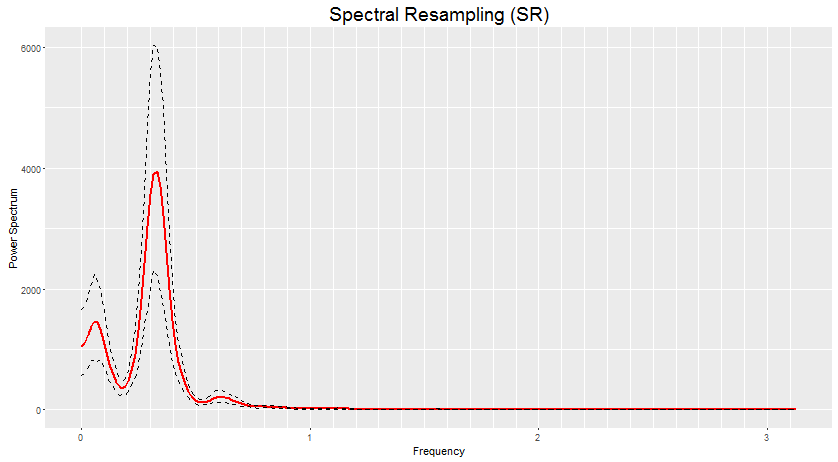
\includegraphics[scale = 0.4]{Plots/SR.png}
\caption{Black line: mean sample SR; Red Lines: 95 \% confidence intervals}
\label{fig:SR.ci}
\end{figure}

It is also useful to have an idea about the distribution of the length estimates for the largest peaks in the spectrum, for the SR method. Therefore we give a function to do this job.

\begin{knitrout}\footnotesize
\definecolor{shadecolor}{rgb}{0.969, 0.969, 0.969}\color{fgcolor}\begin{kframe}
\begin{alltt}
\hlcom{### Function: distribution of the peaks of SR sample.}
\hlcom{#             This function also provides an histogram.}
\hlstd{SR.distribution} \hlkwb{<-} \hlkwa{function}\hlstd{(}\hlkwc{SR.sample}\hlstd{,} \hlkwc{n.peaks}\hlstd{) \{}

  \hlcom{# Checking input}
  \hlkwa{if}\hlstd{(}\hlkwd{class}\hlstd{(SR.sample)} \hlopt{!=} \hlstr{"SR"}\hlstd{)}
    \hlkwd{stop}\hlstd{(}\hlstr{"input not of class SR"}\hlstd{)}

  \hlcom{# This library implement the function findpeaks}
  \hlkwd{library}\hlstd{(pracma)}

  \hlcom{# Setting dimensions and frequency parameters}
  \hlstd{R} \hlkwb{<-} \hlkwd{dim}\hlstd{(SR.sample)[}\hlnum{2}\hlstd{]}
  \hlstd{n.tilda} \hlkwb{<-} \hlkwd{dim}\hlstd{(SR.sample)[}\hlnum{1}\hlstd{]}
  \hlstd{n} \hlkwb{<-} \hlstd{n.tilda} \hlopt{*} \hlnum{2}
  \hlstd{k} \hlkwb{<-} \hlnum{0}\hlopt{:}\hlstd{(n.tilda} \hlopt{-} \hlnum{1}\hlstd{)}
  \hlstd{freq.rad} \hlkwb{<-} \hlnum{2}\hlopt{*}\hlstd{pi}\hlopt{*}\hlstd{k}\hlopt{/}\hlstd{n}

  \hlcom{# Largest peaks in each bootstrap sample}
  \hlstd{counts} \hlkwb{<-} \hlkwd{matrix}\hlstd{(}\hlnum{NA}\hlstd{,} \hlkwc{nrow} \hlstd{= n.peaks,} \hlkwc{ncol} \hlstd{= R)}

  \hlcom{# Getting largest peaks for each bootstrap sample}
  \hlkwa{for}\hlstd{(n} \hlkwa{in} \hlnum{1}\hlopt{:}\hlstd{n.peaks) \{}
    \hlkwa{for}\hlstd{(r} \hlkwa{in} \hlnum{1}\hlopt{:}\hlstd{R) \{}
      \hlstd{counts[n, r]} \hlkwb{<-} \hlstd{freq.rad[}\hlkwd{findpeaks}\hlstd{(SR.sample[, r])[n,} \hlnum{2}\hlstd{]]}
    \hlstd{\}}
  \hlstd{\}}

  \hlcom{# Plotting histogram}
  \hlstd{dat} \hlkwb{<-} \hlkwd{data.frame}\hlstd{(}\hlkwc{counts} \hlstd{=} \hlkwd{c}\hlstd{(counts))}
  \hlstd{p} \hlkwb{<-} \hlkwd{ggplot}\hlstd{(}\hlkwc{data} \hlstd{= dat,}
              \hlkwd{aes}\hlstd{(dat}\hlopt{$}\hlstd{counts))} \hlopt{+}
    \hlkwd{geom_histogram}\hlstd{(}\hlkwc{fill} \hlstd{=} \hlstr{"blue"}\hlstd{,} \hlkwc{col} \hlstd{=} \hlstr{"black"}\hlstd{,} \hlkwc{breaks} \hlstd{=} \hlkwd{seq}\hlstd{(}\hlnum{0}\hlstd{, pi,} \hlkwc{by} \hlstd{=} \hlnum{.04}\hlstd{))} \hlopt{+}
    \hlkwd{coord_cartesian}\hlstd{(}\hlkwc{xlim} \hlstd{=} \hlkwd{c}\hlstd{(}\hlnum{0}\hlstd{, pi))} \hlopt{+}
    \hlkwd{scale_x_continuous}\hlstd{(}\hlkwc{minor_breaks} \hlstd{=} \hlkwd{seq}\hlstd{(}\hlnum{0}\hlstd{, pi,} \hlnum{0.1}\hlstd{))} \hlopt{+}
    \hlkwd{theme}\hlstd{(}\hlkwc{plot.margin} \hlstd{=} \hlkwd{unit}\hlstd{(}\hlkwd{c}\hlstd{(}\hlnum{1}\hlstd{,}\hlnum{1}\hlstd{,}\hlnum{1}\hlstd{,}\hlnum{1}\hlstd{),} \hlstr{"cm"}\hlstd{))} \hlopt{+}
    \hlkwd{xlab}\hlstd{(}\hlstr{"Frequency"}\hlstd{)} \hlopt{+} \hlkwd{ylab}\hlstd{(}\hlstr{"Power Spectrum"}\hlstd{)}

  \hlkwd{return}\hlstd{(}\hlkwd{list}\hlstd{(}\hlkwc{counts} \hlstd{= counts,} \hlkwc{plot} \hlstd{= p))}
\hlstd{\}}
\end{alltt}
\end{kframe}
\end{knitrout}


Figure \ref{fig:SR.ciao} show the distribution of the bootstrap sample for the three largest peaks in the spectrum.


\begin{figure}[htbp]
\centering
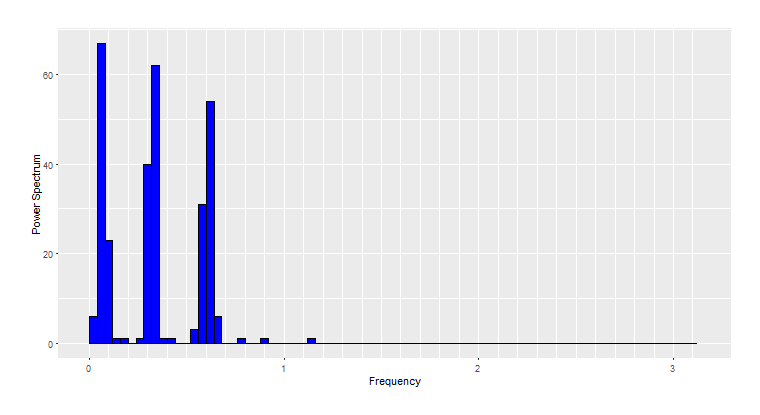
\includegraphics[scale = 0.5]{Plots/SR_distr.png}
\caption{Frequency length estimates for the three largest peaks in spectrum}
\label{fig:SR.ciao}
\end{figure}

\end{document}
